\subsection{Views}	

\subsection{Logic view} 
The logic view provide an overview of the requirements over the principle of the game process. This figure shows a decomposition of the logic of the game process and the relationship between these elements.

\begin{figure}[ht!]
	\centering
	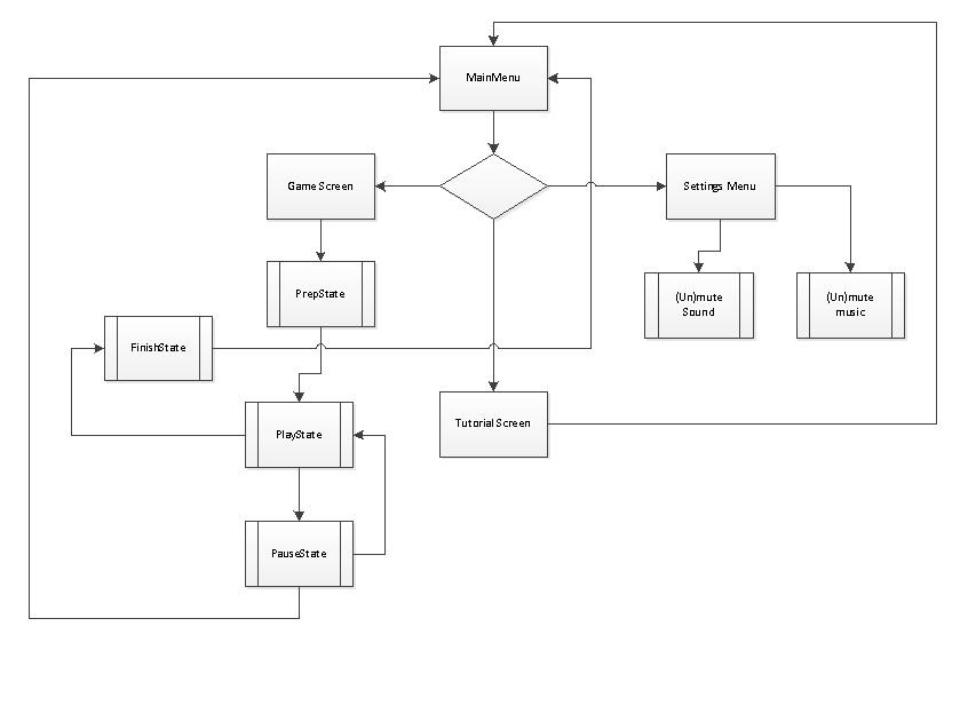
\includegraphics[width=150mm]{viewpoint.jpg}
	\caption{Logic view}
	\label{fig:logicView}
\end{figure}

\newpage
\subsection{Process view}
This activity diagram show the flow between the different action in which state of the game process. Note that this is only a simplified diagram of the playing part of the application. This make it easier to understand the system integrity. The game application start at the main menu. There you will be presented by multiple choice: Play, Tutorial and Settings. Hence by choosing Play you will see that you get to a playscreen for configuration of the gameplay, before starting the game. By following the action of each state you will get a general process view of the game application.


\begin{figure}[ht!]
	\centering
	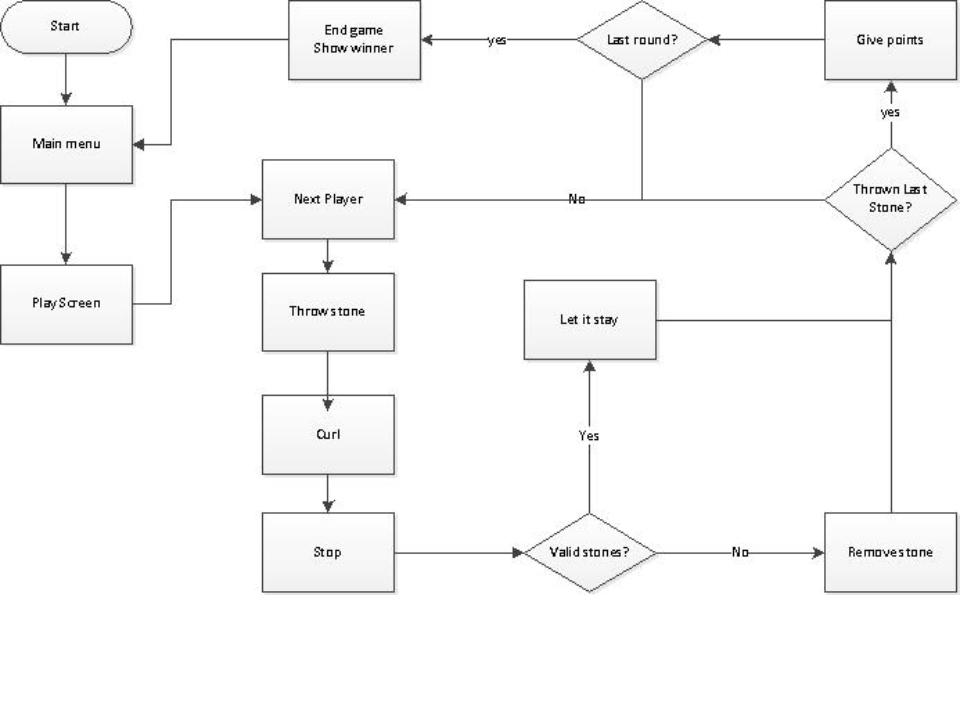
\includegraphics[width=150mm]{view.jpg}
	\caption{Process view}
	\label{fig:processView}
\end{figure}

\newpage
\subsection{Development view}
With the CurlingGame project at the base, it extends into three packages - model, viewactivities and the gamestate. Our model package takes care the model objects, as the curlingstone and the track, and is related to the Game class which draws and updates models. Our gamestate package holds all the viewcontrollers of the project. GameSettings is related to the game to change final variables such as how many balls to play with. Pause/Settings is an activity that pauses the game and brings up a settings-activity on top of the game activity. Finally, the Game class runs, draws, updates, and controls the entire game and other classes. Our project utilizes the Sheep API.\\

\begin{figure}[ht!]
	\centering
	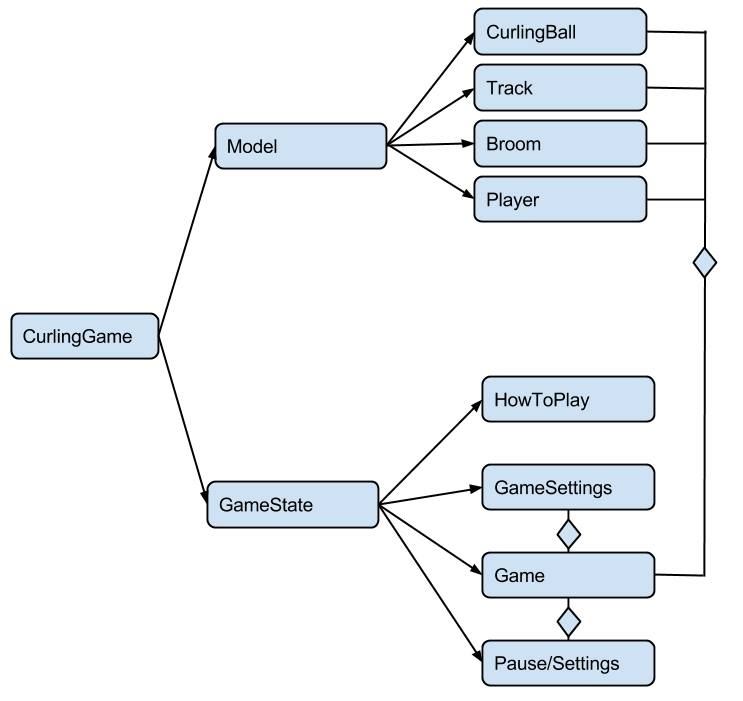
\includegraphics[width=150mm]{development_view.jpg}
	\caption{Development view}
	\label{fig:developmentView}
\end{figure}
\newpage

